\section{Thermodynamik}

\subsection{Terminologie}

\begin{center}
    \begin{tabular}{l||l|lll}
        \textbf{System ist $\downarrow$} & \textbf{Materie-} & & \multicolumn{2}{l}{\textbf{Energietausch}}  \\
			& \textbf{tausch} &	& Arbeit & Wärme \\ \hline
		offen & erlaubt & - & erlaubt  & erlaubt \\
		      &         & adiabatisch  & erlaubt & Nein\\
			  &         & arbeitsdicht & Nein    & erlaubt\\
			  &         & beides       & Nein    & Nein\\ \hline
		geschlossen & Nein & - & möglich  & möglich \\
		      &         & adiabatisch  & möglich & Nein\\
			  &         & arbeitsdicht & Nein    & möglich\\
			  &         & energiedicht & Nein    & Nein\\
	\end{tabular}
\end{center}

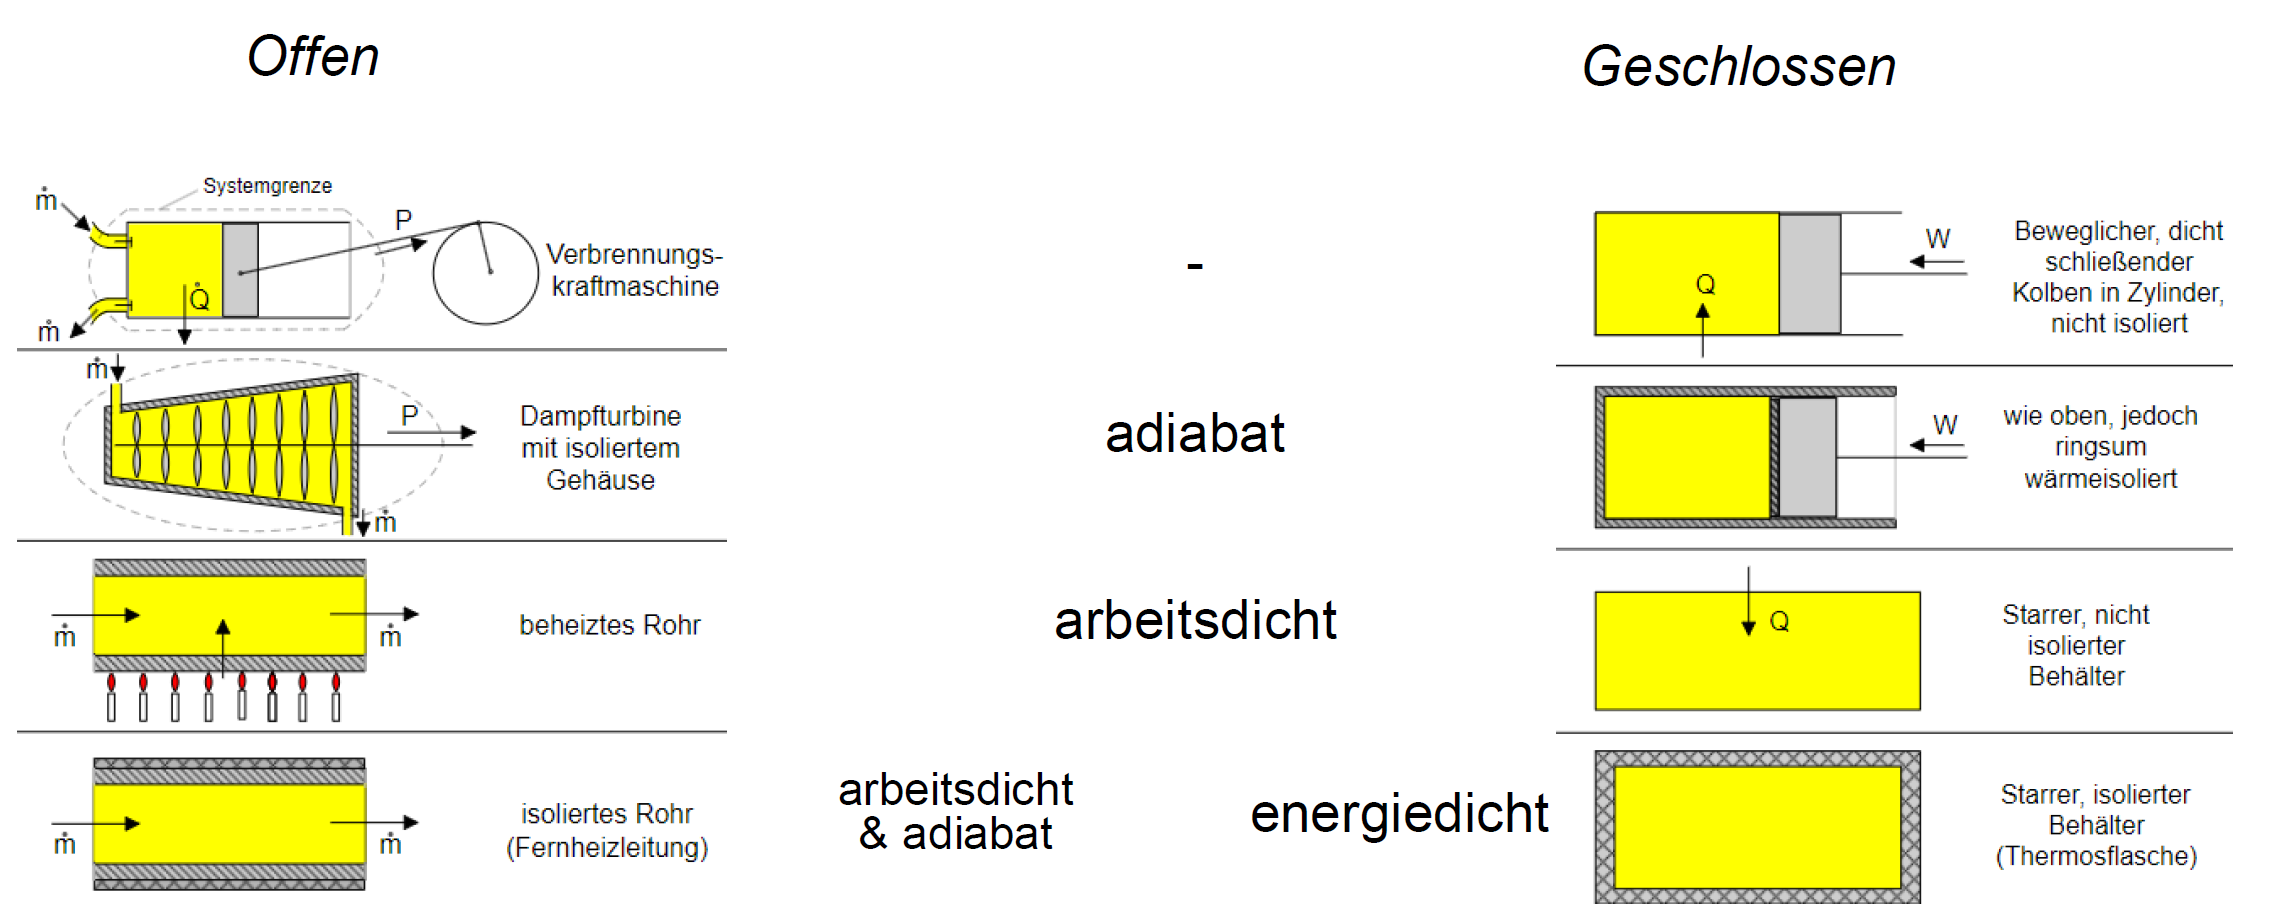
\includegraphics[width=\linewidth]{Bilder/thermodynamisches_system.png}

\subsection{Absolute Temperatur $T$}
$$ \boxed{ T = \theta + 273.15 \, K = \theta - \theta_0 }$$

\begin{tabular}{c l c}
		$T$ & Absolute Temperatur gemessen in Kelvin & $[T] =\mathrm{K}$  \\
		$\theta$ & Temperatur gemessen in °C & $[\theta] = \text{°C}$ \\
		$\theta_0$ & Absoluter Nullpunkt: $= -273.15 \,  \text{°C} = 0 \, \mathrm{K}$  &  \\
\end{tabular}




\subsection{Thermische Ausdehnung}

\subsubsection{Längenausdehnung $\Delta \, l $}

$$ \boxed{  l' = l + \Delta \,  l = l + \alpha \cdot l \cdot \Delta \, T = l\, (1 + \alpha \cdot \Delta \, T ) }$$


\begin{tabular}{c l c}
		$l'$ & Länge nach Ausdehnung & $[l'] = \mathrm{m}$ \\
		$l$ & Anfangslänge & $[l] = \mathrm{m}$ \\
		$\Delta \, l$ & Längenänderung & $[\Delta \, l] = \mathrm{m}$ \\
		\rule{0pt}{8pt}$\alpha$ & Längenausdehnungskoeffizient & $[\alpha] = \mathrm{\frac{1}{K}}$ \\ 
		$\Delta \, T $ & Temperaturänderung & $[\Delta \, T ] = \mathrm{K}$ \\
\end{tabular}


\subsubsection{Flächenausdehnung $\Delta \, A $}

$$ \boxed{ A' = A + \Delta \,  A = A + \underbrace{  \beta }_{\substack{\approx 2 \, \alpha}}  \cdot A \cdot \Delta \, T = A\, (1 + \beta \cdot \Delta \, T ) } $$


\begin{tabular}{c l c}
		$A'$ & Fläche nach Ausdehnung & $[A'] = \mathrm{m^2}$ \\
		$A$ & Anfangsfläche & $[A] = \mathrm{m^2}$ \\
		$\Delta \, A$ & Flächenänderung & $[\Delta \, A] = \mathrm{m^2}$ \\
		\rule{0pt}{8pt}$\beta$ & Flächenausdehnungskoeffizient & $[\beta] = \mathrm{\frac{1}{K}}$ \\ 
		$\Delta \, T $ & Temperaturänderung & $[\Delta \, T ] = \mathrm{K}$ \\
\end{tabular}



\subsubsection{Volumenausdehnung $\Delta \, V $}

$$ \boxed{ V' = V + \Delta \,  V = V + \underbrace{  \gamma }_{\substack{\approx 3 \, \alpha}}  \cdot V \cdot \Delta \, T = V \, (1 + \gamma \cdot \Delta \, T ) }$$


\begin{tabular}{c l c}
		$V'$ & Volumen nach Ausdehnung & $[V'] = \mathrm{m^3}$ \\
		$V$ & Anfangsvolumen & $[V] = \mathrm{m^3}$ \\
		$\Delta \, V$ & Volumenänderung & $[\Delta \, V] = \mathrm{m^3}$ \\
		\rule{0pt}{8pt}$\gamma$ & Volumenausdehnungskoeffizient & $[\gamma] = \mathrm{\frac{1}{K}}$ \\ 
		$\Delta \, T $ & Temperaturänderung & $[\Delta \, T ] = \mathrm{K}$ \\
\end{tabular}

% \vfill\null
% \columnbreak

\begin{center}
    \begin{tabular}{lc}
        \textbf{Material} & \textbf{Koeffizient ($10^{-6} K^{-1} $)}\\ \hline
		Aluminium       & 23 \\
		Eisen           & 12 \\
		Stahl, unlegiert& 11 ... 13 \\
		Diamant         & 1.3 \\
		Silizium        & 2 \\
		Gummi           & 220 \\
		Beton           & 12 \\
		Polysterol      & 70 \\
		Zerodur         & 0 $\pm$ 0.007 \\
	\end{tabular}
\end{center}




\subsection{Thermische Spannung $\sigma$}


$$\boxed{  p = \sigma = \varepsilon \cdot E = E \cdot \frac{\Delta l}{l} =  E \cdot \alpha \cdot \Delta \, T } $$

\begin{tabular}{c l c}
		$\sigma$ & Thermische Spannung & $[\sigma] = \mathrm{Pa}$ \\
		$\varepsilon$ & Dehnung & $[\varepsilon] = 1$ \\
		\rule{0pt}{8pt}$E$ & Elastizitätsmodul & $[E] = \mathrm{\frac{N}{m^2}}$ \\
		\rule{0pt}{8pt}$\alpha$ & Längenausdehnungskoeffizient & $[\alpha] = \mathrm{\frac{1}{K}}$ \\ 
		$\Delta \, T $ & Temperaturänderung & $[\Delta \, T ] = \mathrm{K}$ \\
		$p$ & Druck & $[p] = \mathrm{Pa} $ \\
\end{tabular}






\section{Ideales Gas}

\subsection{Modell des idealen Gases}
\textbf{Jedes Gas ist gleich!} \\


\begin{tabular}{ll}
$1.$ & Moleküle sind Massepunkte (keine Ausdehnung) \\
$2.$ & Stösse sind elastisch (keine zwischenmolekularen Kräfte) \\
& Kein Volumen bei $T = 0$ \\
& Kein Druck bei $T = 0$ \\
\end{tabular}





\subsubsection{Thermische Ausdehnung von Gasen}
\begin{tabular}{ll}
$\bullet$ & Ausdehnung von Gasen ist sehr gross \\
$\bullet$ & Bei \textbf{allen} Gasen ist die Ausdehnung \textbf{gleich} \\
$\bullet$ & Volumen beim Nullpunkt ist \textbf{Null} \\
\end{tabular}


\subsection{Universelle Gasgleichung}
Alle Gase verhalten sich gleich, insbesondere bei gleicher Anzahl Moleküle \\


$$ \boxed{ \frac{p \cdot V}{T} = \, \const } \qquad  \Rightarrow \boxed{ \frac{p_1 \cdot V_1}{T_1} = \frac{p_2 \cdot V_2}{T_2} } $$ 


\begin{tabular}{c l c}
	$p_x$ & \textbf{Absolut-}Druck & $[p_x] = \mathrm{Pa}$ \\
	& Absolut-Druck: $p_0 + p$ \\
	$V_x$ & Volumen & $[V_x] = \mathrm{m^3}$ \\
	$T_x$ & \textbf{Absolut-}Temperatur (in K) & $[T] = \mathrm{K}$ \\
\end{tabular}
	


	
\subsubsection{Boyle-Mariotte}	
\textbf{Das Gesetz gilt nur bei konstanter Temperatur!} \\
$\Rightarrow$ \textbf{Isotherme} Zustandsänderung

$$  \boxed{ p \cdot V = \, \const } \qquad  \Rightarrow  \boxed{ p_1 \cdot V_1 = p_2 \cdot V_2 } $$ 


\vfill\null
\columnbreak


\subsubsection{Gay-Lussac}

\textbf{ Das Gesetz gilt nur bei konstantem Druck!} \\
$\Rightarrow$ \textbf{Isobare} Zustandsänderung

$$  \boxed{ \frac{V}{T} = \; \const } \qquad  \Rightarrow  \boxed{ \frac{V_1}{T_1} = \frac{V_2}{T_2} } $$


	
	
\subsubsection{Gay-Lussac und Amontons}

\textbf{Das Gesetz gilt nur bei konstantem Volumen!} \\
$\Rightarrow$ \textbf{Isochore} Zustandsänderung

$$ \boxed{ \frac{p}{T} = \; \const } \qquad  \Rightarrow \boxed{ \frac{p_1}{T_1} = \frac{p_2}{T_2} }$$


	
\subsection{Universelle Gasgleichung für ideale Gase}\label{Gasgleichung ideal}

$$ \boxed{ p \cdot V = n \cdot R \cdot T = N \cdot k \cdot T }$$
	
	
\begin{tabular}{c l c}
	$p$ & \textbf{Absolut-}Druck & $[p] = \mathrm{Pa}$ \\
	    & Absolut-Druck: $p_0 + p$ & \\
	$V$ & Volumen & $[V] = \mathrm{m^3}$ \\
	$n$ & Mol-Zahl & $[n] = \mathrm{mol}$ \\
	\rule{0pt}{8pt}$R$ & Universelle Gaskonstante: $R = 8.314 \mathrm{\frac{J}{mol \cdot K}}$ & $[R] = \mathrm{\frac{J}{mol \cdot K}} $ \\
	$T$ & \textbf{Absolut-}Temperatur (in K) & $[T] = \mathrm{K}$ \\
	$N$ & Anzahl Moleküle & $[N] = 1$ \\
	\rule{0pt}{8pt}$k$ & Boltzmann-Konstante $k = 1.381 \cdot 10^{-23} \mathrm{\frac{J}{K}}$ & $[k] = \mathrm{\frac{J}{K}}$ \\
\end{tabular}
	
	
	
	
\subsubsection{Zusammenhänge zwischen den Konstanten}
	
$$  \boxed{ R = k \cdot N_A = \frac{N \cdot k}{n} } $$

$$\boxed{ n = \frac{N}{N_A} = \frac{m}{M} = \frac{N \cdot k}{R} } $$
	


\begin{tabular}{c l c}
	\rule{0pt}{8pt}$R$ & Universelle Gaskonstante: $R = 8.314 \mathrm{\frac{J}{mol \cdot K}}$ & $[R] = \mathrm{\frac{J}{mol \cdot K}} $ \\
	\rule{0pt}{8pt}$k$ & Boltzmann-Konstante $k = 1.381 \cdot 10^{-23} \mathrm{\frac{J}{K}}$ & $[k] = \mathrm{\frac{J}{K}}$ \\
	$N$ & Anzahl Moleküle & $[N] = 1$ \\
	\rule{0pt}{8pt}$N_A$ & 	Avogadrokonstante: $N_A = 6.022 \cdot 10^{23} \, \mathrm{\frac{1}{mol}} $ & $[N_A] =  \mathrm{\frac{1}{mol}}$  \\	
	$n$ & Mol-Zahl & $[n] = \mathrm{mol}$ \\
	$m$ & Masse & $[m] = \mathrm{kg}$ \\
	\rule{0pt}{8pt}$M$ & Mol-Masse & $[M] = \mathrm{\frac{kg}{mol}}$ \\
\end{tabular}

% \vfill\null
% \columnbreak


\subsection{Mechanische Arbeit $\Delta W$ von Gasen}
\label{MechArbeit}

Folgende Formel ist für Flüssigkeiten \textbf{nicht} gültig, da diese \\
inkompressibel sind ($\Delta V = 0$)


$$ \boxed{ \Delta W = F \cdot \Delta s = p \cdot A \cdot \Delta s = p \cdot \Delta V } $$
\\

\begin{tabular}{c l c}
	$\Delta W$ & Mechanische Arbeit von Gas & $[\Delta W] = \mathrm{J}$ \\
	$F$ & Kraft & $[F] = \mathrm{N}$ \\
	$\Delta s$ & Wegänderung & $[\Delta s] = \mathrm{m}$ \\
	$p$ & Druck & $[p] = \mathrm{Pa}$ \\
	$A$ & Fläche & $[A] = \mathrm{m^2}$ \\
	$\Delta V$ & Volumenänderung & $[\Delta V] = \mathrm{m^3}$ \\
\end{tabular}



\subsection{Gesetz von Avogadro}
Ein Mol eines Gases nimmt bei Normalbedingungen immer das \\
gleiche Volumen ein (=Molvolumen) \\
\\
Ideale Gase enthalten bei gleichem Druck p und gleicher \\
Temperatur T immer gleich viele Moleküle (im Molvolumen)





\subsection{Molmasse $M$, Molvolumen $V_m$}

Siehe auch \ref{Gasgleichung ideal}\\

Molmasse ist die \textbf{Ordnungszahl} im Periodensystem

$$  \boxed{ n = \frac{m}{M} = \frac{N}{N_A} } $$


Mol-Volumen:

$$ \boxed{ V_m = \frac{V}{n} }$$



\begin{tabular}{c l c}
	$p$ & \textbf{Absolut-}Druck & $[p] = \mathrm{Pa}$ \\
	    & Absolut-Druck: $p_0 + p$ & \\
	$V$ & Volumen & $[V] = \mathrm{m^3}$ \\
	\rule{0pt}{8pt}$R$ & Universelle Gaskonstante: $R = 8.314 \mathrm{\frac{J}{mol \cdot K}}$ & $[R] = \mathrm{\frac{J}{mol \cdot K}} $ \\
	$T$ & \textbf{Absolut-}Temperatur (in K) & $[T] = \mathrm{K}$ \\
	\rule{0pt}{8pt}$N_A$ & 	Avogadrokonstante: $N_A = 6.022 \cdot 10^{23} \, \mathrm{\frac{1}{mol}} $ & $[N_A] =  \mathrm{\frac{1}{mol}}$  \\	
	\rule{0pt}{8pt}$k$ & Boltzmann-Konstante $k = 1.381 \cdot 10^{-23} \mathrm{\frac{J}{K}}$ & $[k] = \mathrm{\frac{J}{K}}$ \\	
	$n$ & Mol-Zahl & $[n] = \mathrm{mol}$ \\
	$m$ & Masse & $[m] = \mathrm{kg}$ \\
	\rule{0pt}{8pt}$M$ & Mol-Masse & $[M] = \mathrm{\frac{kg}{mol}}$ \\
	$N$ & Anzahl Moleküle & $[N] = 1$ \\
	\rule{0pt}{8pt}$V_m$ & Mol-Volumen & $[V_m] = \mathrm{\frac{m^3}{mol}}$ \\
\end{tabular}

% \vfill\null
% \columnbreak



\subsection{Dichte eines Gases $\rho$}

$$ \boxed{ \rho = \frac{m}{V} = \frac{M}{V_m} = \frac{p \cdot M}{R \cdot T} }$$


\begin{tabular}{c l c}
	\rule{0pt}{8pt}$\rho$ & Gas-Dichte & $[\rho] = \mathrm{\frac{kg}{m^3}}$ \\
	$m$ & Masse & $[m] = \mathrm{kg}$ \\
	$V$ & Volumen & $[V] = \mathrm{m^3}$ \\
	\rule{0pt}{8pt}$M$ & Mol-Masse & $[M] = \mathrm{\frac{kg}{mol}}$ \\
	\rule{0pt}{8pt}$V_m$ & Mol-Volumen (22.4 L bei 0 °C und 1000 hPa) & $[V_m] = \mathrm{\frac{m^3}{mol}}$ \\
	\rule{0pt}{8pt}$p$ & \textbf{Absolut-}Druck & $[p] = \mathrm{Pa}$ \\
	    & Absolut-Druck: $p_0 + p$ & \\
	\rule{0pt}{8pt}$R$ & Universelle Gaskonstante: $R = 8.314 \mathrm{\frac{J}{mol \cdot K}}$ & $[R] = \mathrm{\frac{J}{mol \cdot K}} $ \\
	$T$ & \textbf{Absolut-}Temperatur (in K) & $[T] = \mathrm{K}$ \\
\end{tabular}



\subsection{Phänomene von idealen Gasen}

\subsubsection{Annomalie des Wassers}
Die feste Form (Eis) ist leichter als die flüssige Form (Wasser) \\
Die \textbf{grösste Dichte weist Wasser bei 4 °C} auf, nicht beim \\
 Gefrierpunkt von 0 °C \\

$\Rightarrow$ Ein See gefriert somit nur an der Oberfläche. Am Grund des Sees beträgt die Wassertemperatur 4 °C 


\subsubsection{Osmotischer Druck (Zelldruck)}

Grosse Moleküle innerhalb von vielen kleinen Molekülen in einer Flüssigkeit verhalten sich ähnlich wie die Moleküle eines idealen \\ Gases, wenn die Flüssigkeit von einer für die Müleküle \\
halb-durchlässigen (semi-permeabel) Membran umgeben ist.\\
\\
$ \mathrm{Osmotischer \; Druck:} \; p = \frac{n}{V} \cdot R \cdot T  \qquad \mathrm{(ideale \; Gasgleichung)}$



\subsection{Partialdruck $p_i$}
\textbf{Ausgangslage: Gasgemisch (z.B. Luft: Sauerstoff-Stickstoff)} \\
\\

\begin{minipage}{0.48\linewidth}
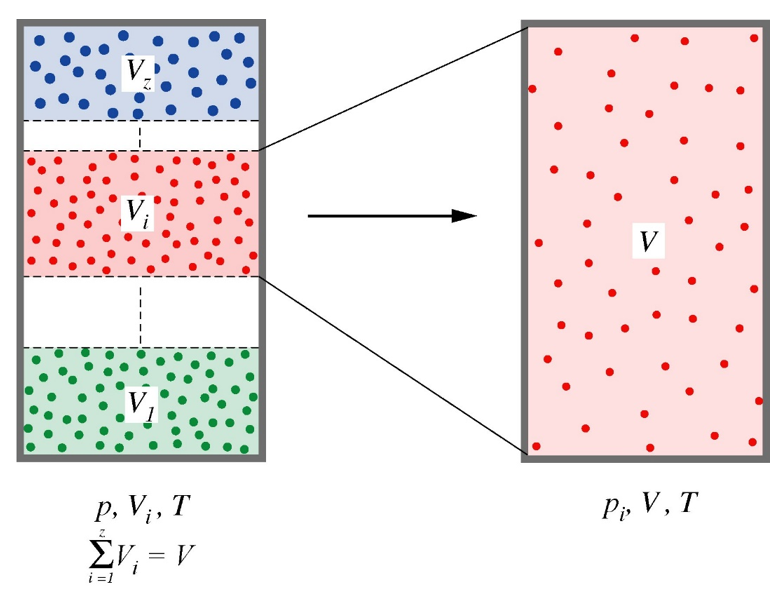
\includegraphics[width=\linewidth]{Bilder/partialdruck}
\end{minipage}
\hfill
\begin{minipage}{0.5\linewidth}
Der Partialdruck $p_i$ ist der Druck, welcher die i-te Gaskomponete erzeugen würde, wenn ihr das gesamte Volumen zur Verfügung stehen würde. \\
\end{minipage}



\subsection{Gesetz von Dalton}
In einem Gas ist die Summe der Partialdrücke $p_i$ gleich dem \\
Gesamtdruck 

$$ \boxed{ \sum_{i=1}^n  p_i = p } $$ 



\begin{tabular}{c l c}
	$p_i$ & Partialdruck & $[p_i] = \mathrm{Pa}$ \\
	$p$ & (Gesamt-) Druck & $[p] = \mathrm{Pa}$ \\
\end{tabular}


\subsection{Volumen- und Massenkonzentration (Gasgemisch)}


\subsubsection{Volumen-Konzentrationen (Volumen-Anteile)}


$$ \boxed{  q_i = \frac{V_i}{V} = \frac{n_i}{n} = \frac{p_i}{p} } $$


\begin{tabular}{c l c}
	$q_i$ & Volumen-Konzentration& $[q_i] = 1$ \\
	$V_i$ & Volumen der i-ten Gas-Komponente & $[V_i] = \mathrm{m^3}$ \\
	$V$ & Gesamt-Volumen & $[V] = \mathrm{m^3}$ \\
	$n_i$ & Molzahl der i-ten Gas-Komponente & $[n_i] = \mathrm{mol}$ \\
	$n$ & Gesamt-Molzahl des Gemischs & $[n] = \mathrm{mol}$ \\
	$p_i$ & Partialdruck der i-ten Gaskomponente & $[p_i] = \mathrm{Pa}$ \\
	$p$ & Druck des Gemischs & $[p] = \mathrm{Pa}$ \\
\end{tabular}






\subsubsection{Massen-Konzentration (Massen-Anteile)}

$$ \boxed{ \mu_i = \frac{m_i}{m} = \frac{M_i}{M} \cdot q_i } $$


\begin{tabular}{c l c}
	$\mu_i$ & Volumen-Konzentrationen & $[\mu_i] = 1$ \\
	$m_i$ & Masse der i-ten Gas-Komponente & $[m_i] = \mathrm{kg}$ \\
	$m$ & Masse der Gemischs & $[m] = \mathrm{kg}$ \\
	\rule{0pt}{8pt}$M_i$ & Mol-Masse der i-ten Gas-Komponete & $[M_i] = \mathrm{\frac{kg}{mol}}$ \\
	\rule{0pt}{8pt}$M$ & Mol-Masse des Gemischs & $[M] = \mathrm{\frac{kg}{mol}}$ \\
	$q_i$ & Volumen-Konzentration& $[q_i] = 1$ \\
\end{tabular}



\subsection{Mol-Masse Gasgemisch}
Die Mol-Masse des Gas-Gemischs kann als gewichteter Mittelwert \\
berechnet werden, gewichtet mit den jeweiligen Volumen-Anteilen  

%\textbf{Die Summe aller $q_i$ muss 1 (bzw. 100%) sein!}


$$ \boxed{ M = \sum_{i=1}^n  q_i \cdot M_i } $$

\begin{tabular}{c l c}
	\rule{0pt}{8pt}$M$ & Mol-Masse Gasgemisch & $[M] = \mathrm{\frac{kg}{mol}} $ \\
	$q_i$ & Volumen-Konzentration& $[q_i] = 1$ \\
	\rule{0pt}{8pt}$M_i$ & Mol-Masse der i-ten Gas-Komponete & $[M_i] = \mathrm{\frac{kg}{mol}}$ \\
\end{tabular}

% \vfill\null
% \columnbreak

\section{Reales Gas}
Im Vergleich zum idealen Gas müssen zwei Dinge berücksichtigt \\
werden: \\


Eigen-Volumen: \\
Ideales Gas hat \textbf{kleineres} Volumen als gemessen \\
(Ideal-Gas-Volumen um das Molekül-Eigenvolumen reduzieren) \\
\\
Binnen-Druck: \\Ideales Gas hat \textbf{grösseren} Druck als gemessen \\
(Ideal-Gas-Druck um Binnendruck erhöhen) 




\subsection{Van der Waals-Gleichung (1 Mol)}
\textbf{$\Rightarrow$ Für nicht-ideale Gase!} 

$$ \boxed{ p' \cdot V'_m = R \cdot T  }$$

$$ \boxed{ p' = p + \frac{a}{V_m^2} }  \qquad \qquad  \boxed{ V'_m = V_m - b }$$


\begin{tabular}{c l c}
	$p'$ & Korrigierter Druck & $[p'] = \mathrm{Pa}$ \\
	\rule{0pt}{10pt}$V'_m$ & Korrigiertes Mol-Volumen & $[V_m] = \mathrm{\frac{m^3}{mol}}$ \\
	\rule{0pt}{10pt}$R$ & Universelle Gaskonstante: $R = 8.314 \mathrm{\frac{J}{mol \cdot K}}$ & $[R] = \mathrm{\frac{J}{mol \cdot K}} $ \\
	$T$ & \textbf{Absolut-}Temperatur (in K) & $[T] = \mathrm{K}$ \\
	$p$ & Druck des Gemischs & $[p] = \mathrm{Pa}$ \\
	\rule{0pt}{10pt}$a$ & Eigenvolumen & $[a] = \mathrm{\frac{J \cdot m^3}{mol^2}}$ \\
	\rule{0pt}{10pt}$b$ & Binnendruck & $[b] = \mathrm{\frac{m^3}{mol}}$ \\
	\rule{0pt}{10pt}$V_m$ & Mol-Volumen & $[V_m] = \mathrm{\frac{m^3}{mol}}$ \\
\end{tabular}

% \vfill\null
% \columnbreak


\subsection{Van der Waals-Gleichung (n Mol)}

$$ \boxed{ \Big(  p + \frac{n^2 \cdot a}{V^2} \Big)  \cdot (V - n \cdot b) = n \cdot R \cdot T } $$



\begin{tabular}{c l c}
	$p$ & Druck des Gemischs & $[p] = \mathrm{Pa}$ \\
	$n$ & Mol-Zahl & $[n] = \mathrm{mol}$ \\
	\rule{0pt}{8pt}$a$ & Eigenvolumen & $[a] = \mathrm{\frac{J \cdot m^3}{mol^2}}$ \\
	$V$ & Volumen & $[V] = \mathrm{m^3}$ \\
	\rule{0pt}{8pt}$b$ & Binnendruck & $[b] = \mathrm{\frac{m^3}{mol}}$ \\
	\rule{0pt}{8pt}$R$ & Universelle Gaskonstante: $R = 8.314 \mathrm{\frac{J}{mol \cdot K}}$ & $[R] = \mathrm{\frac{J}{mol \cdot K}} $ \\
	$T$ & \textbf{Absolut-}Temperatur (in K) & $[T] = \mathrm{K}$ \\
\end{tabular}






\subsubsection{Van der Waals-Parameter}

$$ \boxed{ a = \frac{9}{8} \cdot R \cdot T_k \cdot V_{mk} = \frac{27 R^2 T_k^2}{64 \cdot p_k}}  \qquad \qquad  \boxed{ b = \frac{V_{mk}}{3} = \frac{R T_k}{8 \cdot p_k}}$$


$$ \boxed{ V_{mk} = 3 \cdot b } \quad \quad  \boxed{ T_k = \frac{8 \cdot a}{27 \cdot R \cdot b} } \quad \quad  \boxed{ p_k = \frac{a}{27 \cdot b^2} } $$



\begin{tabular}{c l c}
	\rule{0pt}{8pt}$a$ & Eigenvolumen & $[a] = \mathrm{\frac{J \cdot m^3}{mol^2}}$ \\
	\rule{0pt}{8pt}$R$ & Universelle Gaskonstante: $R = 8.314 \mathrm{\frac{J}{mol \cdot K}}$ & $[R] = \mathrm{\frac{J}{mol \cdot K}} $ \\
	$T_k$ & Kritische \textbf{Absolut-} Temperatur & $[T_k] = \mathrm{K}$ \\
	\rule{0pt}{8pt}$V_{mk}$ & Kritisches Mol-Volumen & $[V_{mk}] = \mathrm{\frac{m^3}{mol}}$ \\
	\rule{0pt}{8pt}$b$ & Binnendruck & $[b] = \mathrm{\frac{m^3}{mol}}$ \\
	$p_k$ & Kritischer Druck & $[p_k] = \mathrm{Pa}$ \\
\end{tabular}



\section{Wärmelehre}

\subsection{Wärme Q}
Wärme ist Energie, welche stets \textbf{(von allein)} von höherer zu \\
niederigerer Temperatur fliesst \\
\\

\begin{tabular}{l c l}
 & $\underleftarrow{1. HS \; 100\%}$ & \\
$\Delta U$ & $=$ & $\Delta W + \Delta Q$ \\
&  $\overrightarrow{2. HS  \; \xout{100\% }}$ & \\
\end{tabular}


\subsection{Erster Hauptsatz der Wärmelehre}
Nicht nur durch Wärmezufuhr, sondern auch durch mechanische \\
Arbeit lässt sich die Temperatur und damit die innere Energie $U$ \\
erhöhen


$$ \boxed{ \Delta U =\Delta W + \Delta Q } $$

\begin{tabular}{c l c}
	$\Delta U$ & Zu-/Abgeführte Innere Energie & $[\Delta U] = \mathrm{J}$ \\
	$\Delta W$ & Zu-/Abgeführte Arbeit & $[\Delta W] = \mathrm{J}$ \\
	& z.B. $\mathrm{E_{kin}, \; E_{pot}, \, W_{Gas}, \; W_{reib} }$ \\
	$\Delta Q$ & Zu-/Abgeführte Wärme & $[\Delta Q] = \mathrm{J}$ \\
\end{tabular}


\subsubsection{Ansätze für 1. HS}

$$ \Delta Q = E_{kin} = \frac{1}{2} \, m \cdot v^2 $$

$$ \Delta Q = E_{pot} = m \cdot g \cdot h $$

$$ \Delta \dot{Q} = \Delta P $$




\subsubsection{Mechanische Arbeit eines Gases}
Für mehr Details, siehe Abschnitt ~\ref{MechArbeit}

$$  \boxed{\Delta W = p \cdot \Delta V } $$





\subsection{Mechanische Wärmeäquivalente}

1 Kalorie = $4,1868 \, \mathrm{J \; (cal)}$ \\
 \quad $\Rightarrow$ Energie, um 1 Gramm Wasser um 1 Grad zu erwärmen \\
 \\
1 kcal = $4186,8 \, \mathrm{J} $ \\
 \quad $\Rightarrow$ Energie, um 1 Kilogramm Wasser um 1 Grad zu erwärmen \\




\subsubsection{Elektrisches Wärmeäquivalent $c$}
\textbf{Elektrische Energie = Wärme}

$$ U \cdot I \cdot t = c \cdot m \cdot \Delta T \quad \Leftrightarrow \quad c = \frac{U \cdot I \cdot t}{m \cdot \Delta T}$$

\begin{tabular}{c l c}
	\rule{0pt}{8pt}$c$ & Elektrisches Wärmeäquivalent & $[c] = \mathrm{\frac{J}{kg \cdot K}}$ \\
	$U$ & Spannung & $[U] = \mathrm{V}$ \\
	$I$ & Strom & $[I] = \mathrm{A}$ \\
	$t$ & Zeit & $[t] = \mathrm{s}$ \\
	$m$ & Masse & $[m] = \mathrm{kg}$ \\
	$\Delta T$ & Temperaturänderung & $[\Delta T] = \mathrm{K}$ \\
\end{tabular}


% \vfill\null
% \columnbreak

\subsection{Wärmekapazität}
Die Wärmekapazität drückt das Energiespeicher-Vermögen aus.

$$ \boxed{ Q = c \cdot m \cdot \Delta T = n \cdot c_M \cdot \Delta T = C \cdot \Delta T  }$$


\subsubsection{Absolute Wärmekapazität $C$}
Energiespeicher-Vermögen eines \textbf{Gegenstands}

$$ \boxed{ \Delta Q = C \cdot \Delta T \quad \quad C\frac{\Delta T}{\Delta t} = \dot{Q}} $$


\subsubsection{Spezifische Wärmekapazität $c$}
Energiespeicher-Vermögen einer \textbf{Substanz}

\begin{minipage}{0.4\linewidth}
	$$ \boxed{ \Delta Q = c \cdot m \cdot \Delta T  } $$	
\end{minipage}
\hfill
\begin{minipage}{0.5\linewidth}
	\begin{center}
		\begin{tabular}{lc}
			\textbf{Substanz} & \textbf{c bei 20°C}\\ \hline
			Wasser      & 4182 \\
			Ethanol     & 2430 \\
			Glyzerin    & 2390 \\
			Quecksilber & 139 \\
			Gold        & 129 \\
			Stahl       & 480 \\
		\end{tabular}
	\end{center}
\end{minipage}

\subsubsection{Molare Wärmekapazität $c_M$}
Energiespeicher-Vermögen einer \textbf{Anzahl Moleküle}

$$ \boxed{ c_M = \frac{c}{n} = M \cdot c } $$


\begin{tabular}{c l c}
	$\Delta Q$ & Zu-/Abgeführte Wärme & $[\Delta Q] = \mathrm{J}$ \\
	\rule{0pt}{8pt}$c$ & spezifische Wärmekapazität & $[c] = \mathrm{\frac{J}{kg \cdot K}}$ \\
	\rule{0pt}{8pt}$c_M$ & molare Wärmekapazität & $[c_M] = \mathrm{\frac{J}{mol \cdot K}}$ \\
	\rule{0pt}{8pt}$C$ & absolute Wärmekapazität & $[C] = \mathrm{\frac{J}{K}}$ \\
	$m$ & Masse & $[m] = \mathrm{kg}$ \\
	$\Delta T$ & Temperaturänderung & $[\Delta T] = \mathrm{K}$ \\
	$n$ & Mol-Zahl & $[n] = \mathrm{mol}$ \\
	\rule{0pt}{8pt}$M$ & Mol-Masse & $[M] = \mathrm{\frac{kg}{mol}}$ \\
\end{tabular}

% \vfill\null
% \columnbreak

\subsubsection{Molare Wärmekapazität von Gasen}

$$ \boxed{ C_{mp} - C_{mV} = R }$$


\begin{tabular}{c l c}
	\rule{0pt}{8pt}$C_{mp}$ & isobare Wärme-Kapazität ($p = \const)$ & $[C_{mp}] = \mathrm{\frac{J}{mol \cdot K}}$ \\
	\rule{0pt}{8pt}$C_{mV}$ & isochore Wärme-Kapazität ($V = \const)$ & $[C_{mV}] = \mathrm{\frac{J}{mol \cdot K}}$ \\
	\rule{0pt}{8pt}$R$ & Universelle Gaskonstante $R = 8.314 \mathrm{\frac{J}{mol \cdot K}}$ & $[R] = \mathrm{\frac{J}{mol \cdot K}} $ \\
\end{tabular}




\subsubsection{Molare Wärmekapazität von Festkörpern}


$$ T > \Theta_D: \quad C_m \approx 3 \, R \approx 25 \frac{J}{mol \cdot K}  \qquad \mathrm{(Dulong-Petit)}$$

$$ T \ll \Theta_D: \quad C_m = \frac{12 \cdot \pi^4}{5}  \cdot R \cdot  \Big( \frac{T}{\Theta_D}  \Big)^3 \qquad \mathrm{(Debye)}  $$


\begin{tabular}{c l c}
	$T$ & \textbf{Absolut-}Temperatur (in K) & $[T] = K$ \\
	$\Theta_D$ & Debye-Temperatur $\Theta_D \approx 200 \, \mathrm{K}$ & $[\Theta_D] = \mathrm{K}$ \\
	\rule{0pt}{8pt}$C_m$ & molare Wärmekapazität & $[C_m] = \mathrm{\frac{J}{mol \cdot K}}$ \\
	\rule{0pt}{8pt}$R$ & Universelle Gaskonstante: $R = 8.314 \mathrm{\frac{J}{mol \cdot K}}$ & $[R] = \mathrm{\frac{J}{mol \cdot K}} $ \\
\end{tabular}






\subsection{Latente Wärme, Enthalpie (Schmelz-/ Verdampfungswärme)}



\begin{minipage}{0.5\linewidth}
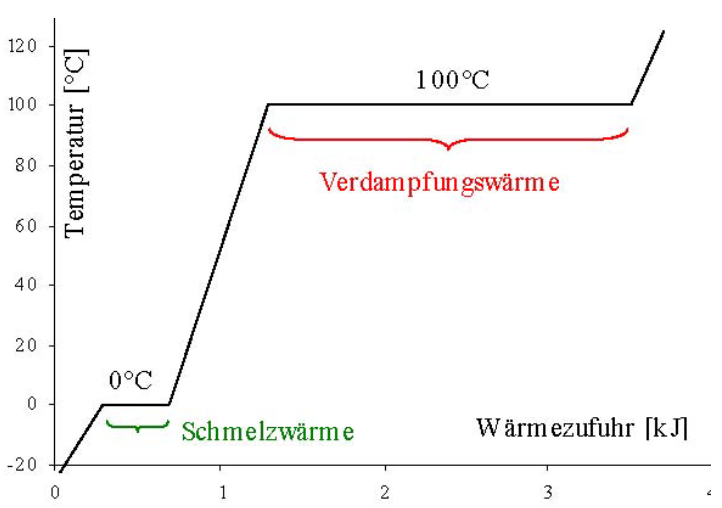
\includegraphics[width=0.99\linewidth]{Bilder/latente_waerme_2}\\
\\
\end{minipage}
\hfill
\begin{minipage}{0.5\linewidth}
Beim Schmelzen und Verdampfen findet \textbf{keine} Temperaturerhöhung statt \\
Beim Gefrieren und oder \\
Kondensieren wird diese \\
versteckte Wärme wieder frei, \textbf{ohne} Abnahme der Temperatur \\
\\
\end{minipage}

\textbf{Die Schmelz-/ Verdampfungswärme ist stark druckabhängig} \\


$$ \boxed{ Q_f = q_f \cdot m } \qquad \qquad q_{f_{Wasser}} := 334 \mathrm{\frac{kJ}{kg}} $$

$$ \boxed{ Q_s = q_s \cdot m } \qquad \qquad q_{s_{Wasser}} := 2256 \mathrm{\frac{kJ}{kg} } $$



\begin{tabular}{c l c}

	$Q_f$ & Schmelz-/Erstarrungs-Wärme & $[Q_f] = \mathrm{J}$ \\
	\rule{0pt}{8pt}$q_f$ & Spezifische Schmelzwärme & $[q_f] = \mathrm{\frac{J}{kg}}$ \\
	$Q_S$ & Verdampfungs-/Kondensations-Wärme & $[Q_S] = \mathrm{J}$ \\
	\rule{0pt}{8pt}$q_s$ & Spezifische Verdampfungs-Wärme& $[q_s] = \mathrm{\frac{J}{kg}}$ \\
	$m$ & Masse & $[m] = \mathrm{kg}$ \\
\end{tabular}




% \vfill\null
% \columnbreak



\subsection{Wärmebilanz}
Wärmeaustausch zwischen verschiedenen Materialien \\

In einem abgeschlossenen System (nach aussen isoliert) muss gelten: \\
\textbf{Zugeführte Wärme = Abgeführte Wärme}

$$  \boxed{ \sum_{i=1}^n  ( \Delta Q_i + \Delta Q_{f_i} + \Delta Q_{s_i} ) = 0 } $$


\begin{tabular}{c l c}
	$\Delta Q_i$ & i-te Wärme-Menge aus & $[\Delta Q_i] = \mathrm{J}$ \\
				& Temperatur-Zu-/Abnahme & \\
	$\Delta Q_{f_i}$ & i-te Wärme-Menge aus  &  $[\Delta Q_{f_i}] = \mathrm{J}$ \\
				& Schmelz-/Erstarrungs-Vorgang  & \\
	$\Delta Q_{s_i}$ & i-te Wärme-Menge aus & $[\Delta Q_{s_i}] = \mathrm{J}$\\
					 & Verdampfungs-/Kondensations-Vorgang &  \\
	& +  zugeführte Wärme-Menge &  \\
	& - abgeführter Wärme-Menge & \\
\end{tabular}




\section{Phasen und Phasenübergänge}


\subsection{Phasen}


\begin{tabular}{ll}
$\bullet$ & \textbf{Fest} \\
		  & feste Gestalt; festes Volumen \\
$\bullet$ & \textbf{Flüssig} \\
		  & keine feste Gestalt; festes Volumen \\
$\bullet$ & \textbf{Gasförmig} \\
		  & keine feste Gesalt; kein festes Volumen \\
$\bullet$ & \textbf{Plasma} \\
		  & Bei sehr hoher Temperatur ist Materie ionisiert (Elektronengas) \\
$\bullet$ & \textbf{Mischung / Dispersion:} \\
\end{tabular}

\begin{center}
	\begin{tabular}{l|cc}
		                   & \textbf{flüssig} & \textbf{gasförmig} \\ \hline
		\textbf{fest}      & Suspension (Sol) & Aerosol (Rauch) \\
		\textbf{flüssig}   & Emulsion & Aerosol (Nebel) \\
		\textbf{gasförmig} & Schaum & - \\
	\end{tabular}
\end{center}






\subsection{Dampfdruck $p_s(T)$}
\textbf{Der Dampfdruck bedeutet das Gleichgewicht der Flüssigkeit mit ihrer Dampfphase} \\

Der Dampfdruck ist das Niveau des kontanten Drucks im\\
2-Phasengebiet eines realen Gases nach van der Waals. \\
\\
Der Dampfdruck ist nur \textbf{temperaturabhängig} \\
\\
Bei Kompression oder Expansion ändert sich der Dampfdruck nicht, sondern der Anteil Flüssigkeit zu Gas muss ändern \\
\\

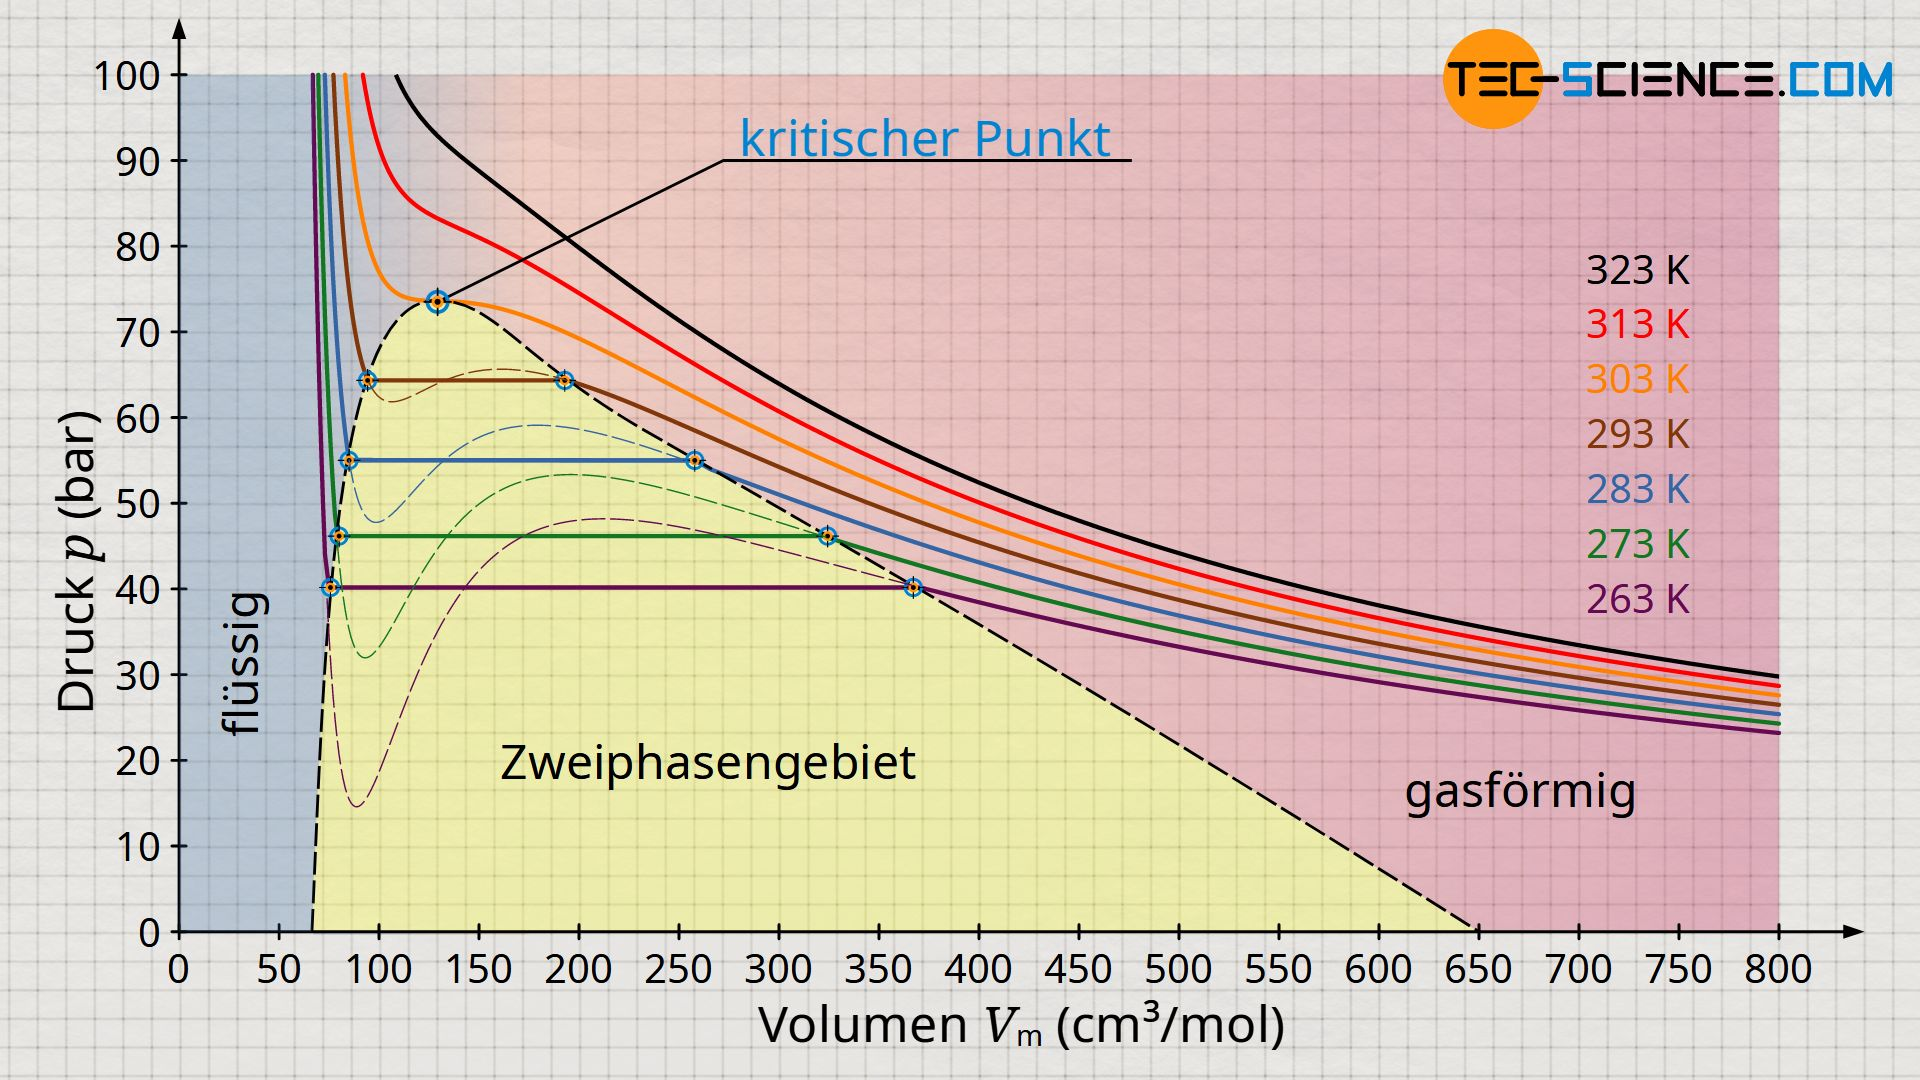
\includegraphics[width=0.9\linewidth]{Bilder/dampfdruck} \\
\\
\textbf{Verdunsten} $\Rightarrow$ Schnellste Teilchen treten aus Flüssigkeit aus \\
\\
\textbf{Sieden/Verdampfen} Dampfdruck = Umgebungsdruck





\subsection{Dampfdruck-Kurve (Clausius-Clapeyron)}

\textbf{Kondensieren $\Leftrightarrow$ Verdampfen}  \qquad flüssig $\Leftrightarrow$ gasförmig  \\

$$ \boxed{ \frac{d \, p_s}{d\, T} = \frac{q_s}{T \cdot  \Big( \frac{1}{\rho_g} - \frac{1}{\rho_f} \Big)  }     } $$



\subsubsection{Dampfdruck $p_s(T)$ von Wasser (Clausius-Clapeyron)}

$$ \boxed{ p_s(T) = p_{s0} \cdot e^{\frac{q_s \cdot M_W}{R} \cdot ( \frac{1}{T_0} - \frac{1}{T}) } } $$

$$ p_{s0} = 610.7 \, \mathrm{Pa} \quad T_0 = 273 \, \mathrm{K} \quad q_s = 2420 \, \mathrm{\frac{kJ}{kg}} \quad M_W = 18.02 \, \mathrm{\frac{g}{mol}}  $$



\subsection{Schmelzdruck-Kurve (Clausius-Clapeyron)}

\textbf{Erstarren $\Leftrightarrow$ Schmelzen}  \qquad fest $\Leftrightarrow$ flüssig \\

$$ \boxed{ \frac{d \, p_f}{d\, T} = \frac{q_f}{T \cdot  \Big( \frac{1}{p_f} - \frac{1}{p_s} \Big)  }     } $$




\subsection{Gasdruck-Kurve (Clausius-Clapeyron)}

\textbf{Desublimieren $\Leftrightarrow$ Sublimieren} \qquad fest $\Leftrightarrow$ gasförmig \\

$$ \boxed{ \frac{d \, p_{sub}}{d\, T} = \frac{q_s + q_f}{T \cdot  \Big( \frac{1}{\rho_g} - \frac{1}{\rho_s} \Big)  }     } $$



\begin{tabular}{c l c}
	\rule{0pt}{10pt}$q_s$ & spezifische Verdampfungs-Wärme & $[q_s] = \mathrm{\frac{J}{kg}}$ \\
	\rule{0pt}{10pt}$q_f$ & spezifische Schmelz-Wärme & $[q_f] = \mathrm{\frac{J}{kg}}$ \\
	$q_s + q_f$ & spezifische Sublimations-Wärme & \\
	$p_s$ & Dampfdruck & $[p_s] = \mathrm{Pa}$ \\
	$p_f$ & Schmelzdruck & $[p_f] = \mathrm{Pa}$ \\
	$p_g$ & Schmelzdruck & $[p_g] = \mathrm{Pa}$ \\
	\rule{0pt}{10pt}$\rho_g$ & Dichte Gas & $[\rho_g] = \mathrm{\frac{kg}{m^3}}$ \\
	\rule{0pt}{10pt}$\rho_f$ & Dichte Flüssgkeit & $[\rho_f] = \mathrm{\frac{kg}{m^3}}$ \\
	\rule{0pt}{10pt}$\rho_s$ & Dichte Festkörper & $[\rho_s] = \mathrm{\frac{kg}{m^3}}$ \\
	$T$ & Temperatur   & $[T] = K$ \\
	$M$ & Molare Masse & $[M] = \frac{kg}{mol}$ \\
	\rule{0pt}{8pt}$R$ & Universelle Gaskonstante: $R = 8.314 \mathrm{\frac{J}{mol \cdot K}}$ & $[R] = \mathrm{\frac{J}{mol \cdot K}} $ \\
\end{tabular}


% \vfill\null
% \columnbreak



\subsection{Formeln von Magnus}
Die Formeln von Magnus dienen der vereinfachten Berechnung des Dampfdrucks von Wasser = Sättigungsdruck 

\subsubsection{Dampfdruck von Wasser $p_s(\theta)$ $(\theta \geq 0 ^{\circ}C)$}


$$ \boxed{ p_s(\theta) = p_{s0} \cdot 10^{ \frac{7.5 \cdot \theta}{\theta + 237}  } } $$



\subsubsection{Schmelzdruck von Wasser $p_s(\theta)$ $ (\theta \leq 0 ^{\circ}C)$}

$$ \boxed{ p_s(\theta) = p_{s0} \cdot 10^{ \frac{9.5 \cdot \theta}{\theta + 265.5} } } $$


\subsubsection{WMO erweiterte Lösung $p_s(\theta)$ $ (-40^{\circ}C < \theta < 50^{\circ}C) $}

$$ \boxed{p_s(\theta) = p_{s0} \cdot \e ^{\left( \frac{17.62 \cdot \theta}{243.04 + \theta} \right)} }$$



\begin{tabular}{c l c}
	$p_s$ & Dampfdruck / Schmelzdruck & $[p_s] = \mathrm{Pa}$ \\
	$p_{s0}$ & Dampfdruck bei $0^{\circ}C$ \quad $p_{s0} = 610.7 \mathrm{Pa} $ & $[p_{s0}] = \mathrm{Pa}$ \\
	$\theta$ & Temperatur & $[\theta] = \text{°C}$ \\
	
\end{tabular}




\subsection{Umkehrformeln von Magnus}

\subsubsection{$\theta(p_s)$ für $p_s \geq p_{s0}$}


$$ \boxed{ \theta(p_s) = \frac{237 \cdot log \big( \frac{p_s}{6.107} \big)  }{7.5 - log \big( \frac{p_s}{6.107} \big)} } $$



\subsubsection{$\theta(p_s)$ für $p_s \leq p_{s0}$}

$$ \boxed{ \theta(p_s) = \frac{265.5 \cdot log \big( \frac{p_s}{p_{s0}} \big)  }{9.5 - log \big( \frac{p_s}{p_{s0}} \big)} } $$




\subsection{Luftfeuchtigkeit}

\subsubsection{Absolute Luftfeuchtigkeit  $f$}

$$ \boxed{ f = \frac{m_W}{V}  } $$



\subsubsection{Relative Luftfeuchtigkeit $f_r$}

$$ \boxed{ f_r = \frac{m_W}{m_S} = \frac{p_D}{p_S} = \frac{p_D}{p_S(\theta)}  } $$



\begin{tabular}{c l c}
	$f$ & Absolute Luftfeuchtigkeit & $[f] = \frac{kg}{m^3}$ \\
	$f_r$ & Relative Luftfeuchtigkeit & $[f_r] = 1$ \\
	$m_W$ & Masse Wasserdampf & $[m_W] = \mathrm{kg}$ \\
	$m_S$ & Masse Wasserdampf bei Sättigung & $[m_S] = \mathrm{kg}$ \\
	$V$ & Volumen & $[V] = \mathrm{m^3}$ \\
	$p_D$ & Partialdruck Wasserdampf & $[p_D] = \mathrm{Pa}$ \\
	$p_S$ & Dampfdruck = Sättigungsdruck Wasserdampf & $[p_s] = \mathrm{Pa}$ \\
	$\theta$ & Temperatur & $[\theta] = \text{°C}$ \\
\end{tabular}


% \vfill\null
% \columnbreak



\subsubsection{Feuchte vs. trockene Luft}

\textbf{Feuchte Luft ist leichter als trockene Luft!}

% $$ \boxed{ \rho_f < \rho_t } \qquad \mathrm{(da} \, M_W < M_L \mathrm{)}$$

$$ \boxed{ \rho_f = \rho_t + \frac{p_D}{RT}(M_W - M_L)} $$

\begin{tabular}{c l c}
	\rule{0pt}{10pt}$\rho_f$ & Dichte feuchte Luft & $[\rho_f] = \mathrm{\frac{kg}{m^3}}$ \\
	\rule{0pt}{10pt}$\rho_t$ & Dichte trockene Luft ($ \frac{p_0 M_L}{RT} $) & $[\rho_t] = \mathrm{\frac{kg}{m^3}}$ \\
	\rule{0pt}{10pt}$p_D$ & Partialdruck Wasserdampf & $[p_D] = \mathrm{Pa}$ \\
	\rule{0pt}{10pt}$T$   & Temperatur & $[T] = K$ \\
	\rule{0pt}{10pt}$M_W$ & Molmasse $H_2O$ (18g/mol) & $[M_W] = \mathrm{\frac{kg}{mol}}$ \\
	\rule{0pt}{10pt}$M_L$ & Molmasse Luft (28.949g/mol) & $[M_L] = \mathrm{\frac{kg}{mol}}$ \\
	\rule{0pt}{10pt}$R$ & Universelle Gaskonstante: $R = 8.314 \mathrm{\frac{J}{mol \cdot K}}$ & $[R] = \mathrm{\frac{J}{mol \cdot K}} $ \\	
\end{tabular}



\subsection{Taupunkts-Temperatur $\theta_d$}
Temperatur, bei welcher 100\% Luftfeuchtigkeit herrscht. \\
\\
Wenn die Taupunkt-Temperatur \textbf{unterschritten} wird, dann \\
kondensiert Wasser.

$$ \boxed{ \theta_d (\theta, f_r) = \frac{237 \cdot \Big( \log(f_r) + \frac{7.5 \cdot \theta}{\theta + 237}    \Big)}{7.5 - \Big( \log(f_r) + \frac{7.5 \cdot \theta }{\theta + 237} \Big) }  }$$


$$ \boxed{ \theta_d (x) = \frac{237 \cdot x}{7.5 - x}    \qquad  \text{mit } \quad    x(\theta, f_r) = \log(f_r) + \frac{7.5 \cdot \theta}{\theta + 237}  }   $$


\begin{tabular}{c l c}
	$\theta_d$ & Taupunkts-Temperatur & $[\theta_d] = \text{°C}$ \\
	$f_r$ & relative Luftfeuchtigkeit & $[f_r] = 1$ \\
	$\theta$ & Temperatur & $[\theta] = \text{°C}$ \\
\end{tabular}




\subsection{Relative Innen-Feuchte $f_{ri}$}

$$ \boxed{ f_{ri} = \frac{p_s(\theta_a)}{p_s(\theta_i)} \cdot f_{ra}  }$$

\begin{tabular}{c l c}
	$f_{ri}$ & relative Feuchte im Inneren & $[f_{ri}] = 1$ \\
	$f_{ra}$ & relative Feuchte der Aussenluft & $[f_{ra}] = \text{1}$ \\
	$p_s(\theta_i)$ & Dampfdruck bei Innentemperatur & $[p_s(\theta_i)] = \mathrm{Pa}$ \\
	$p_s(\theta_a)$ & Dampfdruck bei Aussentemperatur &  $[p_s(\theta_a)] = \mathrm{Pa}$  \\
\end{tabular}



% \vfill\null
% \columnbreak


\section{Kinetische Gas-Theorie} %TODO: Evtl. Folie 6, Seite 5 noch einf¨ügen 

\subsection{Aequipartitionsgesetz}

\textbf{Mittlere kinetische Energie} \\
\\
Idealisierte Annahmen: \\

\begin{tabular}{ll}
1. & Moleküle = Massenpunkte \\
2. & Keine (bzw.) elastische Zusammenstösse \\
3. & Keine Kräfte zwischen den Molekülen\\
4. & Elastischer Stoss gegen Wand \\
5. & Alle Moleküle haben gleiche Geschwindigkeit \\
6. & 1/6 aller Moleküle fliegen gegen eine einzelne Wand \\
\\
\end{tabular}


\begin{minipage}{0.48\linewidth}
$$ \boxed{ \overline{E} = f \cdot \frac{k \cdot T}{2} } $$
\end{minipage}
\hfill
\begin{minipage}{0.48\linewidth}
\begin{tabular}{ll}
f = 3 & 1-atomiges Gas \\
f = 5 & 2-atomiges Gas \\
f = 6 & 3-atomiges Gas \\
\\
\end{tabular}
\end{minipage}


\begin{tabular}{c l c}
	$\overline{E}$ & Mittlere kinetische Energie & $[\overline{E}] = \mathrm{J}$ \\
	$f$ & Freiheitsgrade & $[f] = \text{1}$ \\
	\rule{0pt}{8pt}$k$ & Boltzmann-Konstante $k = 1.381 \cdot 10^{-23} \mathrm{\frac{J}{K}}$ & $[k] = \mathrm{\frac{J}{K}}$ \\
	$T$ & \textbf{Absolute} Temperatur & $[T] = \mathrm{K}$ \\	
\end{tabular}


\subsection{Geschwindigkeiten}

\subsubsection{Mittlere quadratische Geschwindigkeit  $u$}

$$ \boxed{ u = \sqrt{\frac{3 \cdot k \cdot T}{m}} = \sqrt{\frac{3 \cdot R \cdot T}{M}} }  $$


\subsubsection{Mittlere Geschwindigkeit $\overline{v}$}

$$ \boxed{ \overline{v} = \sqrt{\frac{8 \cdot k \cdot T}{\pi m}} = \sqrt{\frac{8 \cdot R \cdot T}{\pi M}} }  $$


\subsubsection{Wahrscheinlichste Geschwindigkeit $v_0$}

$$ \boxed{ v_0 = \sqrt{\frac{2 \cdot k \cdot T}{m}} = \sqrt{\frac{2 \cdot R \cdot T}{M}}  }  $$




\begin{tabular}{c l c}
	\rule{0pt}{8pt}$k$ & Boltzmann-Konstante $k = 1.381 \cdot 10^{-23} \mathrm{\frac{J}{K}}$ & $[k] = \mathrm{\frac{J}{K}}$ \\
	$T$ & \textbf{absolute} Temperatur & $[T] = \mathrm{K}$ \\
	$m$ & Masse des Teilchens & $[m] = \mathrm{kg}$ \\
	$M$ & Molmasse & $[M] = \frac{kg}{mol}$ \\
	\rule{0pt}{10pt}$R$ & Universelle Gaskonstante: $R = 8.314 \mathrm{\frac{J}{mol \cdot K}}$ & $[R] = \mathrm{\frac{J}{mol \cdot K}} $ \\	
\end{tabular}




\subsection{Maxwell-Boltzmann-Verteilung}

$$ \boxed{ f(m, \, T, \, v) = \sqrt{\frac{2 \cdot m^3}{\pi \cdot k^3 \cdot T^3 }}  \cdot v^2 \cdot \e ^{- \frac{m \cdot v^2}{2 \cdot k \cdot T}}  }  $$


\begin{tabular}{c l c}
	$m$ & Masse des Teilchens & $[m] = \mathrm{kg}$ \\
	\rule{0pt}{8pt}$k$ & Boltzmann-Konstante $k = 1.381 \cdot 10^{-23} \mathrm{\frac{J}{K}}$ & $[k] = \mathrm{\frac{J}{K}}$ \\
	$T$ & \textbf{absolute} Temperatur & $[T] = \mathrm{K}$ \\
	\rule{0pt}{8pt}$v$ & Geschwindigkeit & $[v] = \mathrm{\frac{m}{s}}$ \\
\end{tabular}





\subsection{Mittlere freie Weglänge $\overline{\lambda}$}

Gibt an, um welche Strecke sich ein Molekül im Mittel bis zum nächsten Zusammenstoss fortbewegen kann.

$$ \boxed{ \overline{\lambda} = \frac{1}{\sqrt{2}} \cdot \frac{1}{n \cdot (\pi \cdot d^2 )} }  \qquad \text{mit Wirkungsquerschnitt } \sigma = \pi \cdot d^2$$

\begin{tabular}{c l c}
	\rule{0pt}{8pt}$n$ & \textcolor{red}{Molekül-Dichte} & $[n] = \mathrm{\frac{1}{m^3}}$\\	
	$d$ & Molekül-Durchmesser & $[d] = \mathrm{m}$ \\
\end{tabular}




\subsection{Dichtefunktion}
Verteilungsfunktion der mittleren, freien Weglänge 

$$ \boxed{ f(x) = \frac{1}{\overline{\lambda}} \cdot \e^{- \frac{x}{\overline{\lambda}}}  } $$


\subsection{Transportvorgänge}

\subsubsection{Wärmeleitung}
Transport von \textbf{kinetischer Energie} (als Wärme wahrgenommen)

$$ \boxed{ j_Q = - \lambda_Q \cdot \frac{\mathrm{dT}}{\mathrm{dx}} \qquad \quad \lambda_Q = \frac{1}{6} \cdot n \cdot \overline{v} \cdot \overline{\lambda} \cdot f \cdot k }  $$




\subsubsection{Diffusion}
Transport von \textbf{Masse} 


$$ \boxed{ j_D = -D \cdot \frac{\mathrm{dn}}{\mathrm{dx}} \qquad \quad  D = \frac{1}{3} \cdot \overline{v} \cdot \overline{\lambda} }  $$



\subsubsection{Viskosität ($v << v_{therm}$)}
Transport von \textbf{Impuls} 


$$ \boxed{ \tau = - \eta \cdot \frac{\mathrm{dv}}{\mathrm{dx}} \qquad \quad  \eta = \frac{1}{3} \cdot \overline{v} \cdot \overline{\lambda} \cdot \rho }  $$


\begin{tabular}{c l c}
	\rule{0pt}{10pt}$j_Q$ & Wärmestrom & $[j_Q] = \mathrm{\frac{W}{m^2}}$ \\
	\rule{0pt}{10pt}$\lambda_Q$ & Wärmeleitfähigkeit & $[\lambda_Q] = \mathrm{\frac{W}{m \cdot K}}$ \\
	$j_D$ & Diffusionsstrom & $[j_D] = ?$ \\
	\rule{0pt}{10pt}$D$ & Diffusionskonstante & $[D] = \mathrm{\frac{m^2}{s}}$ \\
	$\tau$ & Schubspannung & $[\tau] = \mathrm{N}$ \\
	$\eta$ & Viskosität & $[\eta] = \mathrm{Pa \cdot s}$ \\
	\rule{0pt}{10pt}$n$ & \textcolor{red}{Molekül-Dichte} & $[n] = \mathrm{\frac{1}{m^3}}$\\	
	\rule{0pt}{10pt}$\overline{v}$ & Mittlere Geschwindigkeit & $[\overline{v}] = \mathrm{\frac{m}{s}}$ \\
	\rule{0pt}{10pt}$\overline{\lambda}$ & Mittlere freie Weglänge & $[\overline{\lambda}] = \mathrm{m}$ \\
	$f$ & Anzahl Freiheitsgrade & $[f] = \mathrm{1}$ \\
	\rule{0pt}{10pt}$k$ & Boltzmann-Konstante $k = 1.381 \cdot 10^{-23} \mathrm{\frac{J}{K}}$ & $[k] = \mathrm{\frac{J}{K}}$ \\
	$T$ & \textbf{absolute} Temperatur & $[T] = \mathrm{K}$ \\
	\rule{0pt}{10pt}$\rho$ & Dichte & $[\rho] = \mathrm{\frac{kg}{m^3}}$ \\
\end{tabular}


\section{Temperaturstrahlung}

\begin{tabular}{ll}
$\bullet$ & Wärmestahlung = Berührungslose Übertragung von Wärme \\
$\bullet$ & In Form von elektromagnetischen Wellen ($\lambda$ @ IR) \\
$\bullet$ & Körper absorbiert elektromagn. Strahlung und erhöht \\
		  & seine Temperatur \\ 
          & Jeder Körper mit $T > 0 \, K$ straht Wärme ab (Temp-strahlung) \\
$\bullet$ & Für jede Wellenlänge muss ein Körper gleich viel  \\
		  & Energie abstahlen, wie er zuvor aufgenommen hat!\\
\end{tabular}




\subsection{Strahlungs-Gesetze}


\subsubsection{Stefan-Boltzmann-Gesetz}

\begin{tabular}{ll}
$\bullet$ & Ideal schwarzer Körper (Hohlraum) absoliert  \\
		  & \textbf{alle Wellenlängen zu 100 \%}   \\		
$\bullet$ & Je mehr ein Körper absorbiert, desto mehr muss er \\
		  & emmitieren \textbf{(Energie-Gleichgewicht)}   \\	
		  \\
\end{tabular}

Ein schwarzer Körper (=Hohlraumstrahler) der Temperatur $T$ hat eine totale Abstrahlungs-Leistung \textbf{pro Oberfläche} $K_S$ von: 

$$ \boxed{ K_S = \sigma \cdot T^4 }  $$



\begin{tabular}{c l c}
	\rule{0pt}{10pt}$K_S$ & Schwarzkörper-Emission & $[K_S] = \mathrm{\frac{W}{m^2}}$ \\
	\rule{0pt}{10pt}$\sigma$ & Stefan-Boltzmann-Konstante  & $[\sigma] = \mathrm{\frac{W}{m^2 \cdot K^4}}$\\
	\rule{0pt}{10pt}&  $\sigma = 5.671 \cdot 10^{-8} \, \mathrm{\frac{W}{m^2 \cdot K^4}}$ &  \\ \\
	$T$ & Temperatur & $[T] = \mathrm{K}$ \\
\end{tabular}




\subsubsection{Wien'sches Verschiebungsgesetz}

Verschiebung der maximalen Wellenlänge:

$$ \boxed{ \lambda_{max} \cdot T = \const = b  }  $$

\begin{tabular}{c l c}
	$\lambda_{max}$ & Wellenlängen-Maximum (Planck) & $[\lambda_{max}] = \mathrm{m}$ \\
	$T$ & Temperatur & $[T] = \mathrm{K}$ \\
	\rule{0pt}{8pt}$b$ & Konstante: $b = 2.898 \cdot 10^{-3} \mathrm{ m \cdot K}$ & $ [b] = \mathrm{ m \cdot K}$ \\
\end{tabular}





\subsubsection{Planck'sches Gesetz der Quantenmechanik}

Ein Oszillator, welcher auf ein anderes Energieniveau  \\
(=Elektronen-Kreisbahnen nach Bohr) wechselt, setzt die \\
Energiedifferenz $\Delta E$ in ein Lichtquant (Photon) mit \\
entsprechender Frequenz $f$ um. \\
Je nach Vorzeichen von $\Delta E$ wird das Photon emmitiert  \\
oder absorbiert . \\

$$ \boxed { \Delta E = h \cdot f }  $$

\begin{tabular}{c l c}
	$\Delta E$ & spektrale Abstrahlung (Energie) & $[\Delta E] = \mathrm{J}$ \\
	$h$ & Planck'sches Wirkungsquantum & $[h] = \mathrm{J \cdot s} $\\
	&  $h = 6.628 \cdot 10^{-34} \, \mathrm{J \cdot s}$ &  \\
	\rule{0pt}{8pt}$f$ & Frequenz des Photons & $ [f] = \mathrm{\frac{1}{s} = Hz}$ \\
\end{tabular}



% \vfill\null
% \columnbreak


\subsection{Wärmetransport (an Beispiel Hauswand)}


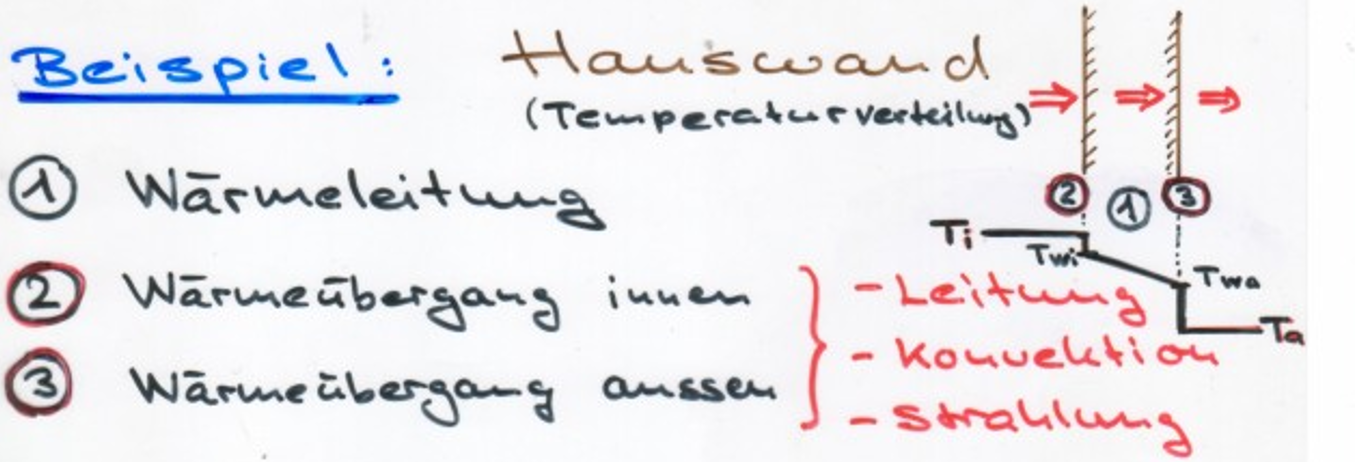
\includegraphics[width=0.9\linewidth]{Bilder/Waermetransport} \\


\subsubsection{Wärmeleitung}

$$ \boxed{ j = - \lambda \cdot \frac{\mathrm{d} T}{\mathrm{d} x}  } $$ 


\begin{tabular}{c l c}
	\rule{0pt}{10pt}$j$ & Wärmestromdiche & $[j] = \mathrm{\frac{W}{m^2}}$ \\
	\rule{0pt}{10pt}$\lambda$ & Wärmeleitfähigkeit & $[\lambda] = \mathrm{\frac{W}{m \cdot K}} $\\
	\rule{0pt}{10pt}$\frac{\mathrm{d} T}{\mathrm{d} x}$ & Wärmeabnahme / Gradient & $ [\frac{\mathrm{d} T}{\mathrm{d} x}] = \mathrm{\frac{T}{m}}$ \\
\end{tabular}


\subsubsection{Wärmeübergang}

$$ \boxed{\mathrm{innen:} \quad  j = \alpha_i \cdot (T_i - T_{wi} )  \qquad \mathrm{mit} \, \alpha_i = 8 \mathrm{\frac{W}{m^2 \cdot K}}  }  $$ 

$$ \boxed{\mathrm{aussen:} \quad  j = \alpha_a \cdot (T_{wa} - T_a )  \qquad \mathrm{mit} \, \alpha_a = 20 \mathrm{\frac{W}{m^2 \cdot K}}  }  $$ 





\subsubsection{Wärmedurchgang}
Material + Dicke zusammengefasst (\textbf{Bereich von $k$ beachten!!})

$$ \boxed{ j = k \cdot (T_i - T_a) = k \cdot \Delta T  \qquad \mathrm{mit} \, k = \frac{\lambda}{d} }  $$ 



\begin{tabular}{c l c}
	\rule{0pt}{10pt}$j$ & Wärmestromdiche & $[j] = \mathrm{\frac{W}{m^2}}$ \\
	\rule{0pt}{10pt}$\lambda$ & Wärmeleitfähigkeit & $[\lambda] = \mathrm{\frac{W}{m \cdot K}} $\\
	\rule{0pt}{10pt}$\frac{\mathrm{d} T}{\mathrm{d} x}$ & Wärmeabnahme / Gradient & $ [\frac{\mathrm{d} T}{\mathrm{d} x}] = \mathrm{\frac{T}{m}}$ \\
	\rule{0pt}{10pt}$\alpha_i$ & Wärmeübergangszahl innen & $[\alpha_i] = \mathrm{\frac{W}{m^2 \cdot K}} $\\
	\rule{0pt}{10pt}$\alpha_a$ & Wärmeübergangszahl aussen & $[\alpha_a] = \mathrm{\frac{W}{m^2 \cdot K}} $\\
	$T_{wa}$ & Temperatur Wand aussen & $[T_{wa}] = \mathrm{K}$ \\
	$T_a$ & Aussentemperatur & $[T_a] = \mathrm{K}$ \\
	$T_{wi}$ & Temperatur Wand innen & $[T_{wi}] = \mathrm{K}$ \\
	$T_i$ & Innentemperatur & $[T_i] = \mathrm{K}$ \\
	\rule{0pt}{10pt}$k$ & Wärmedurchgangszahl & $[k] = \mathrm{\frac{W}{m^2 \cdot K}}$ \\
	$d$ & Dicke der Wand & $[d] = \mathrm{m}$ \\
	\\
\end{tabular}


$$ \textcolor{orange}{  \boxed{ P =  \dot{Q} = j \cdot A } } \quad \text{siehe auch \ref{Wärmeleistung}} $$




% \vfill\null
% \columnbreak



\subsubsection{Wärmedurchgang komplett}

Der komplette Wärmedurchgang leitet sich her durch die \textbf{Erhaltung der Wärmestrondichte $j$} und errechnet sich mit:

% $$ \boxed{\mathrm{2 \; Schichten:} \quad \frac{1}{k_{12}} = \frac{1}{k_1} + \frac{1}{k_2} }  $$  

$$ \boxed{\mathrm{n \; Schichten:} \quad \frac{1}{k_{tot}} = \frac{1}{\alpha_i} + \sum_x  \frac{1}{k_x} + \frac{1}{\alpha_a}  }  $$

$$ \boxed{\mathrm{zylindrisch:} \quad \frac{1}{k_{tot}} = r_a \Big(  \frac{1}{\alpha_i \cdot r_i} + \sum_x \frac{1}{\lambda_x} \cdot \ln \big( \frac{r_{xa}}{r_{xi}} \big)  + \frac{1}{\alpha_a \cdot r_a} \Big) }  $$




\begin{tabular}{c l c}
	\rule{0pt}{10pt}$k_x$ & Wärmedurchgangszahl x-te Schicht & $[k_x] = \mathrm{\frac{W}{m^2 \cdot K}}$ \\
	\rule{0pt}{10pt}$\alpha_i$ & Wärmeübergangszahl innen & $[\alpha_i] = \mathrm{\frac{W}{m^2 \cdot K}} $\\
	\rule{0pt}{10pt}$\alpha_a$ & Wärmeübergangszahl aussen & $[\alpha_a] = \mathrm{\frac{W}{m^2 \cdot K}} $\\
	$r_i$ & Innenradius Rohr & $[r_i] = \mathrm{m}$	 \\
	$r_a$ & Aussenradius Rohr & $[r_a] = \mathrm{m}$	 \\
	\rule{0pt}{10pt}$\lambda_x$ & Wärmeleitfähigkeit & $[\lambda] = \mathrm{\frac{W}{m \cdot K}} $\\
\end{tabular}





\subsection{Wärme-Bedarf (Heizleistung)}\label{Wärmeleistung}
Der Wärme-Bedarf (=Heizleistung) setzt sich zusammen aus \textbf{Wärmeverlust durch Wärmeleitung} und durch \textbf{Wärmeverlust durch Luftaustausch}: 

$$\mathrm{\underbrace{W"armeverlust}_{\substack{\dot{Q}}}  = \underbrace{Heizleistung}_{\substack{P}}  }   $$

$$ \boxed{ P = \dot{Q}_{tot} = \dot{Q}_W + \dot{Q}_L }   $$

\begin{minipage}{0.46\linewidth}
$$ \boxed{ \dot{Q}_W = A \cdot j = A \cdot k \cdot \Delta T  }$$ \\
\end{minipage}
\hfill
\begin{minipage}{0.46\linewidth}
$$ \boxed{ \dot{Q}_L = c_L \cdot \rho_L \cdot \dot{V} \cdot \Delta T}   $$
\\
\end{minipage}



$$ \boxed{ \mathrm{allgemein: } \quad \dot{Q}_{tot} = \sum_{i=1}^n  \big[  (A_i \cdot k_i + c_L \cdot \rho_L \cdot \dot{V} ) \cdot \Delta T \big]  }   $$


\begin{tabular}{c l c}
	\rule{0pt}{10pt}$\dot{Q}_{tot}$ & Totaler Wärmeverlust & $[\dot{Q}_{tot}] = \mathrm{\frac{J}{s} = W}$ \\
	\rule{0pt}{10pt}$\dot{Q}_W$ & Wärmeleistung & $[\dot{Q}_W] = \mathrm{\frac{J}{s} = W}$ \\
	\rule{0pt}{10pt}$\dot{Q}_L$ & Luftaustausch & $[\dot{Q}_L] = \mathrm{\frac{J}{s} = W}$ \\
	\rule{0pt}{10pt}$k_i$ & Wärmedurchgangszahl i-te Schicht & $[k_i] = \mathrm{\frac{W}{m^2 \cdot K}}$ \\
	\rule{0pt}{10pt}$\dot{V}$ & Volumenstrom ($\dot{V} = \frac{V}{t}$) & $[\dot{V}] = \mathrm{\frac{m^3}{s}}$ \\
	\rule{0pt}{10pt}$\rho_L$ & Dichte der Luft: $\rho_L = 1.2 \, \mathrm{\frac{kg}{m^3}}$ & $[\rho_L] = \mathrm{\frac{kg}{m^3}}$ \\
	\rule{0pt}{10pt}$c_L$ & Wärmekapazität Luft: $c_L = 1000 \, \mathrm{\frac{J}{kg \cdot K}}$ & $[c_L] = \mathrm{\frac{J}{kg \cdot K}}$ \\
	$A$ & Fläche der Wärmeleitung & $[A] = \mathrm{m^2}$ \\
	$\Delta T$ & Temperaturdifferenz & $[\Delta T] = \mathrm{K}$ \\
\end{tabular}



% \vfill\null
% \columnbreak



\subsection{Wärmeverlust durch Abstrahlung}

Durch Strahlung kann auch Wärme übertragen werden.

$$ \boxed{ j_{12} = c_{12} \cdot (T_1^4 - T_2^4) = \sigma \cdot \varepsilon \cdot (T_1^4 - T_2^4) }   $$



\begin{tabular}{c l c}
	\rule{0pt}{10pt}$j_{12}$ & W-Transport durch Strahlungsaustausch & $[j_{12}] = \mathrm{\frac{W}{m^2}}$ \\
	\rule{0pt}{10pt}$c_{12}$ & Strahlungsaustauschzahl & $[c_{12}] = \mathrm{\frac{W}{m^2 \cdot K^4}}$ \\
	\rule{0pt}{10pt}$\sigma$ & Stefan-Boltzmann-Konstante  & $[\sigma] = \mathrm{\frac{W}{m^2 \cdot K^4}}$\\
	\rule{0pt}{10pt}&  $\sigma = 5.671 \cdot 10^{-8} \, \mathrm{\frac{W}{m^2 \cdot K^4}}$ &  \\
	\rule{0pt}{10pt}$\varepsilon$ & Emissionsverhältnis & $[\varepsilon] = 1$ \\
\end{tabular}








\subsection{Zustandsänderungen}

$$ \mathrm{Erinnerung \; 1. \; Hauptsatz}: \quad  \Delta U = \Delta W + \Delta Q $$


\subsubsection{Isotherm}
\textbf{bei konstanter Temperatur}

\begin{minipage}{0.48\linewidth}
$$ \boxed{ W_{ab} = n \cdot R \cdot T \cdot \ln \Big( \frac{V_1}{V_2}  \Big) }  $$
\end{minipage}
\hfill
\begin{minipage}{0.48\linewidth}
$$ \boxed{ \Delta Q_{zu} = W } \quad  (\Delta U = 0) $$
\end{minipage}



\subsubsection{Isobar}
\textbf{bei konstantem Druck} \\

\begin{minipage}{0.48\linewidth}
$$ \boxed{ W_{ab} = p \cdot (V_2 -V_1)  }  $$
\end{minipage}
\hfill
\begin{minipage}{0.48\linewidth}
$$ \boxed{ \Delta Q_{zu} = n \cdot C_{mp} \cdot \Delta T } $$
\end{minipage}


\subsubsection{Isochor}
\textbf{bei konstantem Volumen}

\begin{minipage}{0.4\linewidth}
$$ \boxed{ W = 0 }  $$
\end{minipage}
\hfill
\begin{minipage}{0.58\linewidth}
$$ \boxed{ \Delta Q_{zu} = n \cdot C_{mV} \cdot \Delta T }  \quad  (\Delta U = \Delta Q) $$
\end{minipage}


\subsubsection{Adiabatisch}
\textbf{ohne Wärme-Austausch} \\


\begin{minipage}{0.58\linewidth}
$$ \boxed{ W_{ab} = n \cdot C_{mV} \cdot \Delta T = c \cdot m \cdot \Delta T}  $$
\end{minipage}
\hfill
\begin{minipage}{0.38\linewidth}
$$ \boxed{ \Delta Q = 0} $$
\end{minipage}



% \vfill\null
% \columnbreak


\section{Rückwandlung innerer Energie}

\subsection{Zweiter Hauptsatz der Wärmelehre}
Innere Energie kann \textbf{nicht zu 100 \%} in Arbeit umgesetzt werden \\
$\Rightarrow$ Carnot-Wirkungsgrad ist der theoretisch höchstmögliche. \\
\\
Wärme kann niemals \underline{von selbst} von einem kälteren Ort zu einem wärmeren Ort fliessen (Clausius)\\
\\
Es gibt keine \underline{periodisch wirkende} Maschine, die nichts anderes bewirkt als Erzeugung mechanischer Arbeit und Abkühlung eines Wärme-Reservoirs (Kelvin) \\
$\Rightarrow$ Es gibt kein Perpetuum mobile 2. Art


\subsection{Kreisprozess (reversibler Prozess)}
$$ \text{Anfangszustand} \; = \; \text{Endzustand} $$ 


\begin{minipage}{0.48\linewidth}
\textbf{Rechts}laufender Kreisprozess \\
\\
\begin{tabular}{ll}
$\bullet$ & Gibt Arbeit ab\\
$\bullet$ & \textcolor{blue}{Wärmekraftmaschine} \\
$\bullet$ & Bei hoher $T$ wird Wärme  \\
		  & aus Prozess \textbf{zu}geführt\\
$\bullet$ & Nur Bruchteil der Wärme \\
		  & in Arbeit verwandelbar \\
$\bullet$ & Obergrenze: \\
		  & Carnot-Wirkungsgrad\\

\end{tabular}
\end{minipage}
\hfill
\begin{minipage}{0.48\linewidth}
\textbf{Links}laufender Kreisprozess \\
\\
\begin{tabular}{ll}
$\bullet$ & Verbraucht Arbeit \\
$\bullet$ & \textcolor{violet}{Wärmepumpe} \\
$\bullet$ & Bei hoher $T$ wird dem \\
		  & Prozess Wärme\textbf{ab}geführt\\
$\bullet$ & Erzeugt mehrfaches an \\
		  & Wärme \\
$\bullet$ & Obergrenze: \\
		  & Inv. Carnot-Wirkungsgrad \\
\end{tabular}
\end{minipage}








\subsection{Carnot-Wirkungsgrad}


$$ \boxed{\text{\textcolor{blue}{Wärmekraftmaschine: } }  \quad n_C = \frac{W_{ab}}{Q_{zu}} = \frac{T_{hoch}-T_{tief}}{T_{hoch}} }  $$


$$ \boxed{\text{ \textcolor{violet}{Wärmepumpe:}} \quad  n_{iC} = \frac{Q_{zu}}{W_{ab}} = \frac{T_{hoch}}{T_{hoch}-T_{tief}} }  $$



\begin{tabular}{c l c}
	$n_C$ & Carnot-Wirkungsgrad & $[n_C] = \mathrm{1}$ \\
	$n_{iC}$ & Inverset Carnot-Wirkungsgrad & $[n_{iC}] = \mathrm{1}$ \\
	$T_{tief}$ & Temperatur des Warm-Reservoirs & $[T_{tief}] = \mathrm{K}$ \\
	$T_{hoch}$ & Temperatur des Kalt-Reservoirs & $[T_{hoch}] = \mathrm{K}$  \\
	$Q_{zu}$ & zugeführte Wärme & $[Q_{zu}] = \mathrm{J}$ \\ 
	$W_{ab}$ & abgeführte Energie & $[W_{ab}] = \mathrm{J}$ \\ 
\end{tabular}





% \vfill\null
% \columnbreak


\subsection{Adiabaten-Gleichung (Kreisprozess)}
Adiabate wird beschrieben im pV- / TV- / Tp-Diagramm
\\


\begin{minipage}{0.6\linewidth}
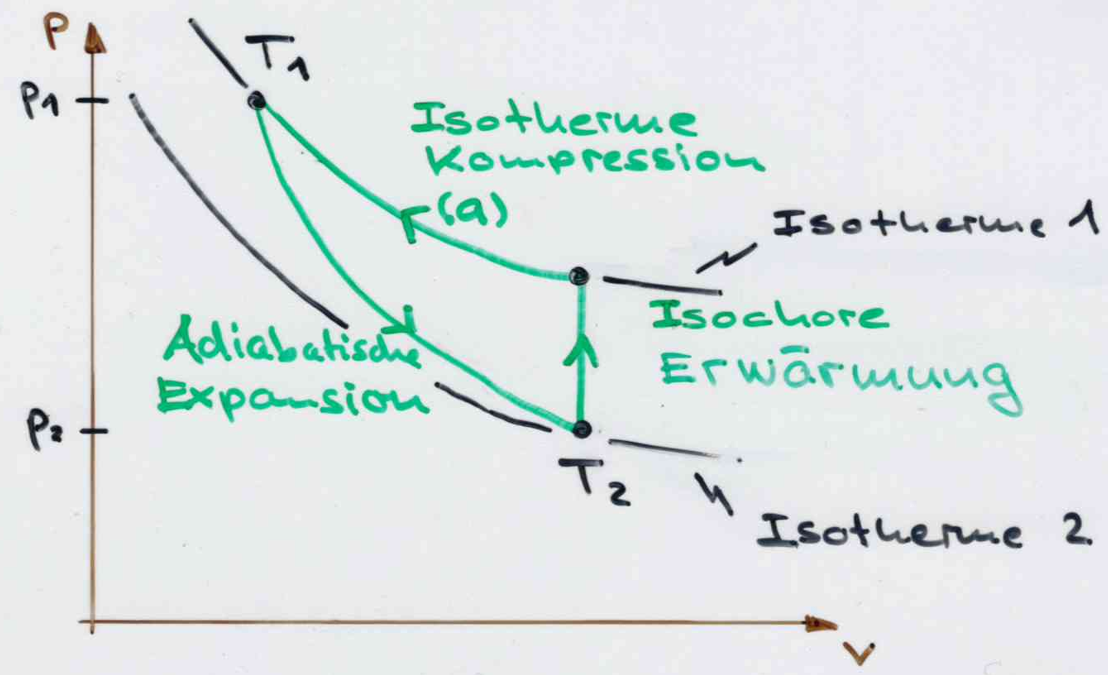
\includegraphics[width=\linewidth]{Bilder/kreisprozess}
\end{minipage}
\hfill
\begin{minipage}{0.38\linewidth}
$$ \boxed{ p \cdot V^\kappa  = \const } $$
$$ \boxed{ T \cdot V^{\kappa -1} = \const } $$
$$ \boxed{ T^\kappa \cdot p^{1-\kappa} = \const } $$
$$ \kappa = \frac{C_{mp}}{C_{mV}}$$
$$ \boxed{ C_{mp} - C_{mV} = R }$$
\\
\end{minipage}




\begin{tabular}{c l c}
	\rule{0pt}{10pt}$C_{mp}$ & Molare Wärmekapazität @ $p = \const$ & $[C_{mp}] = \mathrm{\frac{J}{mol \cdot K}}$ \\
	\rule{0pt}{10pt}$C_{mV}$ & Molare Wärmekapazität @ $V = \const$  & $[C_{mV}] = \mathrm{\frac{J}{mol \cdot K}}$ \\
	\rule{0pt}{10pt}$\kappa$ & Adiabaten-Exponent & $[\kappa] = 1$ \\
	\rule{0pt}{10pt}$R$ & Universelle Gaskonstante $R = 8.314 \mathrm{\frac{J}{mol \cdot K}}$ & $[R] = \mathrm{\frac{J}{mol \cdot K}} $ \\
\end{tabular}



\subsection{Kreisprozesse (Vorgänge)}


\begin{tabular}{lll}
isotherme Expansion & liefert Wärme & benötigt Energie \\
isotherme Kompression & benötigt Wärme & liefert Energie \\
\\
adiabatische Expansion & liefert Arbeit & ohne Wärme \\
adiabatische Kompression & benötigt Arbeit & ohne Wärme \\
\\
isochore Erwärmung & ohne Arbeit & benötigt Wärme \\
isochore Abkühlung & ohne Arbeit & liefert Wärme \\

\end{tabular}


\subsection{Beispiel Kreisprozess}
\begin{minipage}{0.48\linewidth}
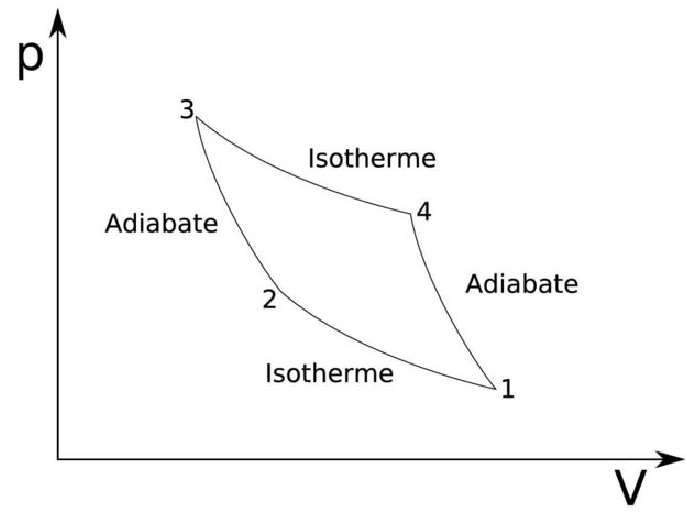
\includegraphics[width=\linewidth]{Bilder/kreisprozess_2} \\
\end{minipage}
\hfill
\begin{minipage}{0.48\linewidth}
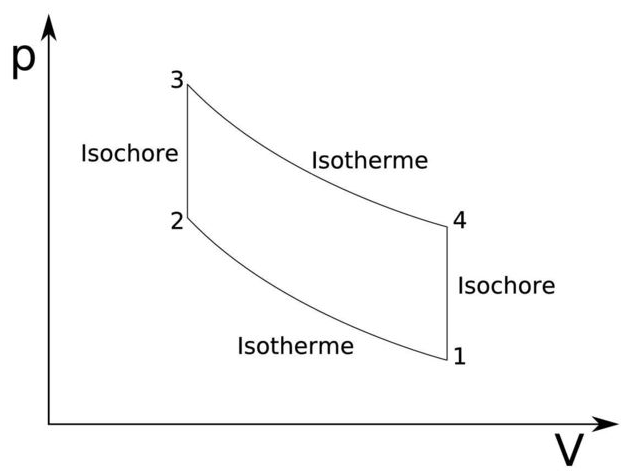
\includegraphics[width=\linewidth]{Bilder/kreisprozess_3} \\
\end{minipage}



% \vfill\null
% \columnbreak


\subsection{Entropie-Zunahme}

\subsubsection{Definition der Entropie-Zunahme}

$$ \Delta S = S_1 + S_2 = \int \frac{1}{T} \, \mathrm{d}Q  $$


\subsubsection{Boltzmann-Gleichung für Entropie-Zunahme}

$$ \boxed{ \Delta S = k \cdot \ln(W) }$$



\begin{tabular}{c l c}
	\rule{0pt}{10pt}$\Delta S$ & Entropie & $[\Delta S] = \mathrm{\frac{J}{K}}$ \\
	\rule{0pt}{10pt}$k$ & Boltzmann-Konstante $k = 1.381 \cdot 10^{-23} \mathrm{\frac{J}{K}}$ & $[k] = \mathrm{\frac{J}{K}}$ \\
	$W$ & Wahrscheinlichkeit eines Zustands & $[W] = 1$ \\
\end{tabular}


\subsubsection{Abgeschlossenes System}

\begin{tabular}{ll}
$ \Delta S \geq 0$ & Entropie kann nur zunehmen in abgeschl. System \\

$ \Delta S > 0$ & Irreversibler Prozess \\

$ \Delta S = 0$ & Reversibler Prozess \\
\end{tabular}

\section{Molmassen wichtiger Atome}

\begin{tabular}{c | c | c }
\textbf{Symbol} & \textbf{Molekül} & \textbf{Molmasse} \\
\hline
\rule{0pt}{10pt} H & Wasserstoff & $1.008 \, \mathrm{\frac{g}{mol}}$ \\
\rule{0pt}{10pt} C & Kohlenstoff & $12.011 \, \mathrm{\frac{g}{mol}}$ \\
\rule{0pt}{10pt} N & Stickstoff & $14.007 \, \mathrm{\frac{g}{mol}}$ \\
\rule{0pt}{10pt} O & Sauerstoff & $15.999 \, \mathrm{\frac{g}{mol}}$ \\
\rule{0pt}{10pt} Al & Aluminium & $26.982 \, \mathrm{\frac{g}{mol}}$ \\
\rule{0pt}{10pt} Si & Silicium & $28.982 \, \mathrm{\frac{g}{mol}}$ \\
\end{tabular}
